\documentclass[12pt, a4paper]{article}

\usepackage[margin=2.5cm]{geometry}
\usepackage{graphicx}
\usepackage{amsmath}
\usepackage{amssymb}
\usepackage{booktabs}
\usepackage{hyperref}
\usepackage{listings}
\usepackage{xcolor}
\usepackage{caption}
\usepackage{subcaption}
\usepackage{parskip}
\usepackage{titlesec}
\usepackage{fancyhdr}

\hypersetup{
    colorlinks=true,
    linkcolor=blue!60!black,
    urlcolor=blue!60!black,
}

\lstset{
    language=Python,
    basicstyle=\ttfamily\small,
    keywordstyle=\color{blue!70!black}\bfseries,
    commentstyle=\color{gray},
    stringstyle=\color{orange!80!black},
    breaklines=true,
    frame=single,
    backgroundcolor=\color{gray!8},
    numbers=left,
    numberstyle=\tiny\color{gray},
    xleftmargin=1.5em,
    framexleftmargin=1.5em,
}

% Marker for the parts that are still to be written.
\newcommand{\todo}[1]{%
    \par\medskip\noindent
    \fcolorbox{red!60!black}{red!5}{%
        \parbox{\dimexpr\linewidth-2\fboxsep-2\fboxrule}{%
            \textbf{\color{red!60!black}TO DO:} #1}}%
    \par\medskip}

\pagestyle{fancy}
\fancyhf{}
\rhead{Collective Robotics -- Tutorial 5}
\lhead{Gandhi, Machida}
\cfoot{\thepage}

\title{
    \vspace{-1cm}
    \textbf{Collective Robotics -- Tutorial 5}\\[0.3em]
    \large Collective Decision-Making: Urn Model, Global Switching, Foraging\\[0.5em]
    \normalsize Hochschule Bonn-Rhein-Sieg\\
    Prof.\ Dr.\ Javad Ghofrani
}
\author{Bhavesh Gandhi \and Jaqueline Machida}
\date{12.07.2026}

\begin{document}

\maketitle
\thispagestyle{fancy}
\tableofcontents
\newpage

% =============================================================================
\section{The Shared Locust Simulation}
% =============================================================================

Tasks 1 and 2 both use the continuous-space, discrete-time locust model of
tutorial 4, task 1.  The locusts live on a ring of circumference $C$, move left
($v = -\text{speed}$) or right ($v = +\text{speed}$), and flip direction in one
of two situations: when the majority of the locusts inside their perception
range $r$ move the opposite way, or spontaneously with probability $P$ per time
step.  The switching rules are unchanged from tutorial 4; only the parameters
differ.  Because both tasks need the same simulation, it lives in a single
module, \texttt{locust.py}, which both import:

\begin{lstlisting}
from locust import simulate
L = simulate(N=50, T=120, C=0.5, speed=0.01, r=0.045, p=0.15, seed=0)
# -> array of left-goer counts L_t, length T + 1
\end{lstlisting}

Two changes to the tutorial-4 code were necessary.

\paragraph{The ring circumference was hard-coded.}
The old \texttt{step()} computed the wrap-around distance as
\texttt{np.minimum(distances, 1 - distances)} and seeded the positions with
\texttt{np.random.uniform(0, 1, n)}.  Both silently assume $C = 1$.  Tutorial 5
uses $C = 0.5$, which would have placed half of the locusts off the ring and
computed the wrong arc distances for the rest.

\paragraph{The simulation was too slow.}
Task 1 requires $5000$ independent runs and task 2 requires runs of $200{,}000$
time steps, which the original per-locust Python loop cannot deliver in
reasonable time.  The loop is replaced by a pairwise distance matrix and a
single matrix--vector product.  Since every locust lies inside its own
perception range, the self-contribution is removed by subtraction rather than by
building an $N \times N$ identity mask:
\[
    \text{net\_dir}_i \;=\; \sum_{j} \mathbb{1}\!\left[d_{ij} < r\right] s_j - s_i ,
    \qquad s_j \in \{-1, +1\}.
\]
Profiling showed that the $N \times N$ distance matrix dominates the runtime and
that in \texttt{float64} it spills out of the L2 cache at $N = 150$: the cost per
step jumped by a factor of six between $N = 100$ and $N = 150$, far more than the
$O(N^2)$ scaling predicts.  The matrix is therefore built in \texttt{float32},
where the rounding error ($\sim 10^{-7}$) is negligible against $r = 0.045$,
while the positions themselves stay \texttt{float64} so that the position
integration does not drift over millions of steps.  A single $N = 50$, $T = 120$
run now takes $6$~ms.

\paragraph{Verification.}
The vectorised majority rule was checked to agree \emph{exactly} with the
tutorial-4 implementation on $200$ random swarm states, and the distribution of
the final left-goer count agrees between the two implementations under a
two-sample Kolmogorov--Smirnov test ($p = 0.93$).  The spontaneous flip rate was
measured at $0.1494$ against the nominal $P = 0.15$.

\newpage
% =============================================================================
\section{Task 1 -- Urn Model for the Locust Scenario}
% =============================================================================

\todo{This section is written together with the task~1 implementation.  It
should describe the measurement of $\Delta L(L)$: simulate for $100$ burn-in
steps so the swarm settles into a stable collective pattern, then record
$\Delta L = L_t - L_{t-1}$ for $t \in [101, 120]$, bin each value by $L_{t-1}$,
and average over ${\approx}5000$ independent runs.  Parameters: $C = 0.5$,
speed $= 0.01$, $r = 0.045$, $N = 50$, $P = 0.15$.  The simulation is already
available as \texttt{locust.simulate()}; see Section~1 for its interface and for
the parameters it takes.}

\subsection{Subtask a -- The Function \texorpdfstring{$\Delta L(L)$}{Delta L(L)}}

\todo{Plot the measured $\Delta L(L)$.  Then discuss the mathematical and
domain-specific meaning of the positions $L^*$ with $\Delta L(L^*) = 0$: they
are the fixed points of the averaged one-step dynamics, i.e.\ the values of $L$
at which the swarm has, on average, no tendency to move either way.
Distinguish the two \emph{stable} fixed points (the consensus states, near
$L = 0$ and $L = N$, where the swarm has agreed on a direction) from the
\emph{unstable} one (the symmetric, undecided state near $L = N/2$, which the
swarm leaves at the slightest perturbation).  Note that the unstable fixed point
is exactly the barrier whose crossing task~2 measures.}

\subsection{Subtask b -- Fitting the Swarm Urn Model}

The urn model from the lecture, with the scaling constant $c$ introduced by the
task sheet, is
\begin{align}
    P_{FB}(s, \varphi) &= \varphi \sin(\pi s), \label{eq:pfb} \\
    \Delta s(s) &= 4c \left(P_{FB}(s, \varphi) - \frac{1}{2}\right)
                          \left(s - \frac{1}{2}\right), \label{eq:ds}
\end{align}
where $P_{FB}$ is the probability of positive feedback, $s = L/N$ is the
fraction of left-goers and $\varphi \in [0, 1]$ is the feedback intensity.

\todo{Fit Equation~\eqref{eq:ds} to the measured data, i.e.\ find $c$ and
$\varphi$, keeping $\varphi$ inside $[0, 1]$.  Report the fitted values and how
the fit was obtained.  Remember that the data are $\Delta L$ against $L$, while
the model is $\Delta s$ against $s$; convert with $s = L/N$ and
$\Delta s = \Delta L / N$.}

\subsection{Subtask c -- Data, Fit and Probability of Positive Feedback}

\todo{Plot the measured data together with the fitted $\Delta s(s)$, and plot the
resulting $P_{FB}(s, \varphi)$ from Equation~\eqref{eq:pfb}.  Discuss what can be
said about the results: how well the idealised urn model reproduces the measured
dynamics, where it deviates (in particular near $s = 0$ and $s = 1$, and near
the fixed points), and what the fitted $\varphi$ says about the strength of the
positive feedback in this swarm.}

\newpage
% =============================================================================
\section{Task 2 -- Density-Dependent Global Switching}
% =============================================================================

\subsection{Overview}

In the biological system, a locust swarm that has converged on one direction
occasionally switches to the other, and it does so more often at low density.
We test whether the simulation of Section~1 reproduces this.  We use the task-1
parameter set ($C = 0.5$, speed $= 0.01$, $r = 0.045$, $P = 0.15$) and vary only
the swarm size, $N \in [20, 150]$.

Three zones are defined on the number of left-goers $L$:
\[
    \text{Zone A: } L > 0.7N, \qquad
    \text{Zone B: } 0.3N \le L \le 0.7N, \qquad
    \text{Zone C: } L < 0.3N .
\]
A \emph{global switch} is a traversal of zone B that connects zone A to zone C,
or zone C to zone A.  While the swarm sits in A or C the counter is zero;
entering B starts it; leaving B into the opposite zone stores the counter and
resets it; leaving B back into the zone it came from resets the counter without
storing it.  The source code is in \texttt{task\_2/task\_2.py}.

\subsection{Implementation}

The zone bookkeeping is implemented as a pure function of the left-goer sequence
$L_t$, which made it possible to test it against hand-constructed sequences
whose correct answer is known: a single A$\to$C crossing, a failed crossing that
returns to its zone of origin, two crossings in opposite directions, a direct
A$\to$C jump with no time spent in B, and an incomplete crossing at the end of a
run.

One case is not specified by the task sheet: a run may \emph{begin} inside zone
B, in which case there is no zone of origin to compare against.  We do not count
such a traversal until the swarm has first touched A or C.

Each of the $10$ swarm sizes is simulated $10$ times for $200{,}000$ time steps,
i.e.\ $2 \times 10^6$ time steps per swarm size.  This is far more than the
$5{,}000$ steps the sheet asks for, and it is necessary: at $N = 150$ a run of
$5{,}000$ steps produces no switch at all.  All swarm sizes use the same number
of time steps, so the switch \emph{counts} are directly comparable across $N$.

\subsection{Two Different Quantities}

The counter defined by the task sheet measures the time the swarm spends
\emph{inside zone B} during a successful crossing.  That is not the same as the
time \emph{between} switches, and it turns out that only the latter carries the
density dependence.  We therefore report both:

\begin{itemize}
    \item the \textbf{crossing time}, i.e.\ the counter as defined above, and
    \item the \textbf{waiting time}, i.e.\ the number of time steps between two
          consecutive switches, measured within each run.
\end{itemize}

\begin{table}[h]
\centering
\begin{tabular}{rrrr}
\toprule
$N$ & \textbf{Switches} & \textbf{Crossing time} & \textbf{Waiting time} \\
\midrule
$20$  & $16759$ & $11.8 \pm 7.4$ & $119 \pm 113$ \\
$30$  & $7100$  & $13.1 \pm 6.5$ & $281 \pm 247$ \\
$40$  & $4485$  & $12.6 \pm 5.2$ & $445 \pm 374$ \\
$50$  & $3476$  & $11.9 \pm 3.9$ & $575 \pm 457$ \\
$65$  & $2094$  & $11.0 \pm 2.9$ & $950 \pm 815$ \\
$80$  & $881$   & $11.3 \pm 2.4$ & $2252 \pm 2261$ \\
$95$  & $312$   & $10.9 \pm 2.1$ & $6211 \pm 6839$ \\
$110$ & $100$   & $11.2 \pm 2.0$ & $19001 \pm 22705$ \\
$130$ & $27$    & $11.3 \pm 1.9$ & $46127 \pm 33865$ \\
$150$ & $2$     & $12.5 \pm 0.5$ & --- \\
\bottomrule
\end{tabular}
\caption{Global switching over swarm size.  Switch counts are per
         $2 \times 10^6$ time steps ($10$ runs of $200{,}000$ steps each).
         Times are mean $\pm$ standard deviation, in time steps.  At $N = 150$
         only two switches were observed and no single run contained two of
         them, so no waiting time can be reported.}
\label{tab:task2}
\end{table}

\begin{figure}[h]
    \centering
    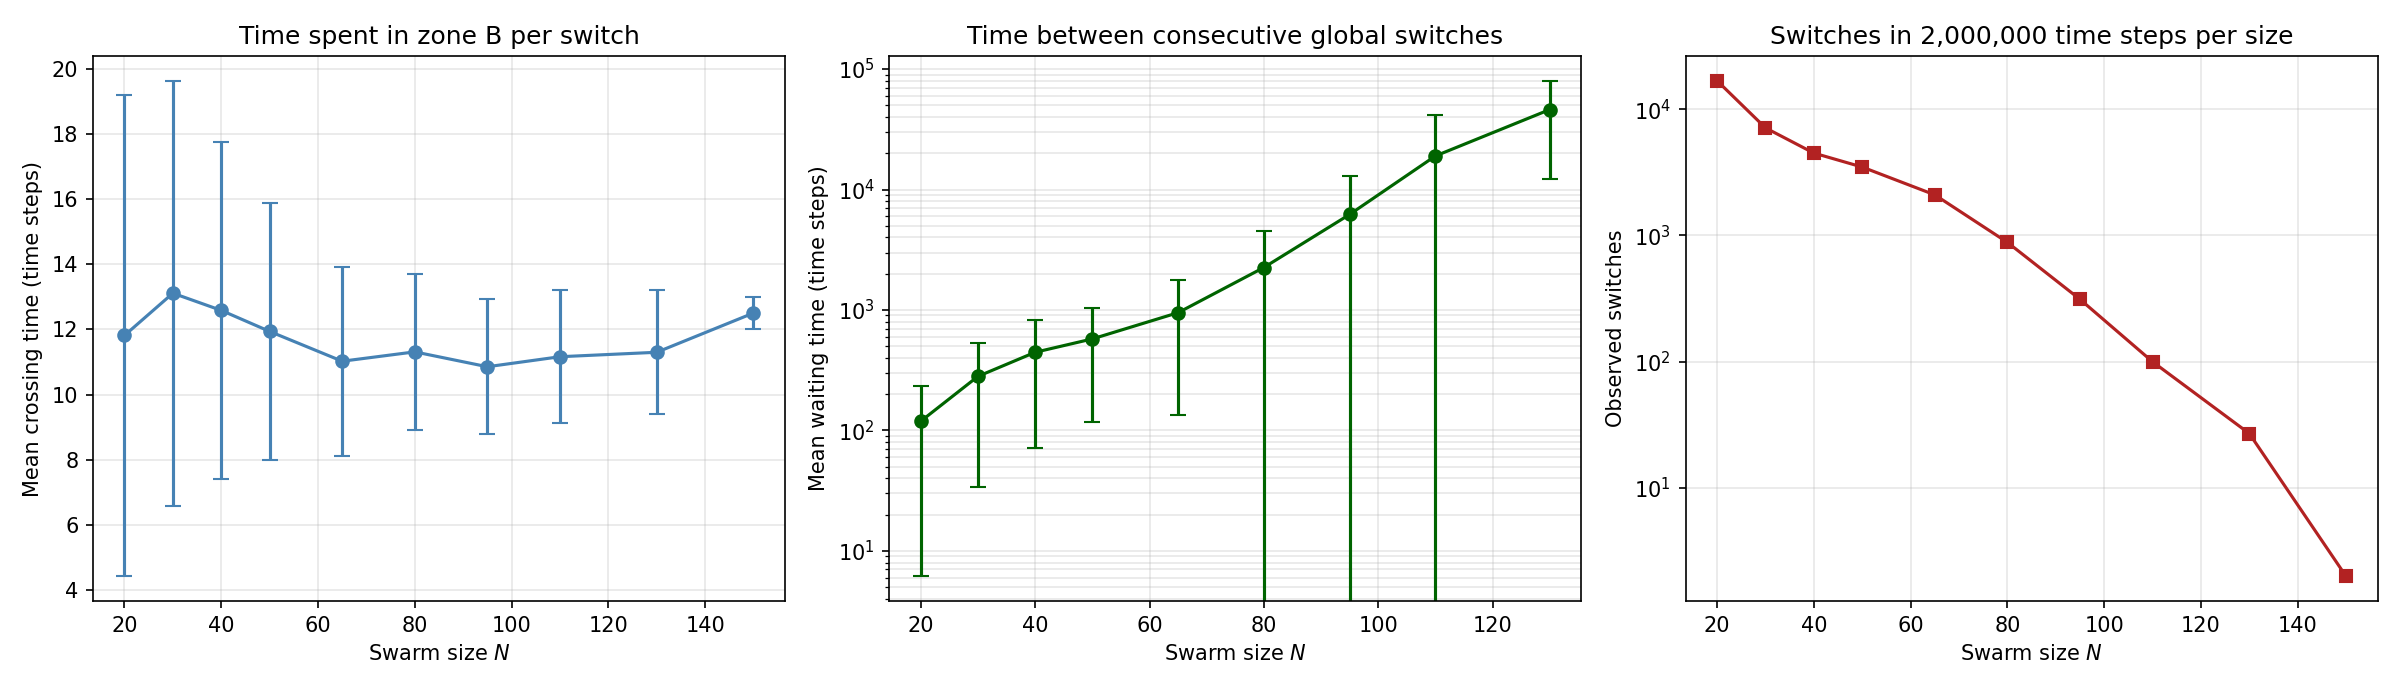
\includegraphics[width=\textwidth]{task_2/plots/task_2_switching.png}
    \caption{Left: mean crossing time, i.e.\ the time spent in zone B per
             switch.  Middle: mean waiting time between consecutive switches
             (logarithmic axis).  Right: number of observed switches per swarm
             size (symmetric-log axis).  Error bars are one standard deviation.}
    \label{fig:task2}
\end{figure}

\subsection{Results and Discussion}

\paragraph{The crossing time is flat.}
The time spent inside zone B per switch stays at $11$--$13$ time steps for every
swarm size (Figure~\ref{fig:task2}, left).  This is the quantity the task
sheet's counter measures, and it shows essentially no density dependence.  The
interpretation is that zone B is not a state the swarm lingers in: once the
swarm is disordered enough that $0.3N \le L \le 0.7N$, it falls into one of the
two consensus attractors in about the same number of steps regardless of how
many locusts there are.  What changes with density is not how quickly the swarm
crosses, but how often it manages to enter the crossing at all.

\paragraph{The waiting time grows steeply.}
The time between consecutive switches grows from $119$ time steps at $N = 20$ to
$46{,}127$ at $N = 130$, a factor of about $390$ (Figure~\ref{fig:task2},
middle; note the logarithmic axis).  Equivalently, the number of switches
observed in a fixed budget of $2 \times 10^6$ time steps collapses from
$16{,}759$ at $N = 20$ to $2$ at $N = 150$ (Figure~\ref{fig:task2}, right).  The
standard deviation of the waiting time is comparable to its mean, as expected
for the roughly exponentially distributed waiting time of a rare escape event.

\paragraph{Do we observe the same as in the natural swarm?}
Yes.  A sparse swarm flips its collective direction constantly; a dense swarm
locks into whichever direction it happened to choose and almost never leaves it.
The mechanism is visible directly in the model.  Alignment is driven by the
local majority, so a locust surrounded by more neighbours is more strongly
pinned to the consensus.  A global switch requires enough locusts to defect
\emph{at the same time} to carry $L$ across the whole of zone B against that
pinning, and the only source of defection is the spontaneous flip, which each
locust performs independently with probability $P = 0.15$.  The probability that
a sufficient number of independent flips coincide falls off very quickly as $N$
grows, which is exactly the steep growth of the waiting time observed above.

This is the same escape-from-a-potential-well picture that underlies the urn
model of task~1: the unstable fixed point at $L^* \approx N/2$ is the barrier
separating the two consensus states, and for large swarms it becomes effectively
insurmountable.

\newpage
% =============================================================================
\section{Task 3 -- Foraging}
% =============================================================================

\subsection{Overview}

We implement a foraging controller for ARGoS\,3 foot-bots.  The robots search a
$4 \times 4$~m arena for objects, push them into a home zone marked by a bright
light, and return to search again.  Swarm performance is measured as the number
of objects collected in a fixed period, for swarm sizes $N \in \{1, \dots, 10\}$.
The simulator configuration, the Lua controller, the C\texttt{++} loop functions
and the analysis scripts live in \texttt{task\_3/}; the whole toolchain runs
inside a single Docker image.

The home zone is a bright yellow light at $(-1.75, 0)$.  Forty objects --
movable cylinders, each carrying a blue LED so that the robots' cameras can see
them -- start in the eastern part of the arena, away from home, so that they
have to be transported.  Each swarm size was run $20$ times for $300$ simulated
seconds, giving $200$ runs in total.

\subsection{Implementation}

\subsubsection{Emulating the bumper}

The task sheet specifies a bumper sensor that measures a force from which the
robot can tell how many objects it is pushing.  ARGoS has no such sensor, so it
is emulated from the proximity ring and the omnidirectional camera.  We first
measured, on this ARGoS build, what an object straight ahead of a robot reads:

\begin{table}[h]
\centering
\begin{tabular}{lrrrr}
\toprule
\textbf{Distance to object} & $16.5$~cm & $19$~cm & $25$~cm & $35$~cm \\
\midrule
\textbf{Proximity reading}  & $1.00$    & $0.37$  & $0.11$  & $0.00$ \\
\bottomrule
\end{tabular}
\caption{The proximity ring fires well before the robot is in contact.  Contact
         occurs at $16.5$~cm: the foot-bot radius ($8.5$~cm) plus the cylinder
         radius ($8$~cm).}
\label{tab:prox}
\end{table}

The bumper is therefore \emph{pressed} when the proximity reading exceeds $0.35$
(the object is then within ${\approx}19$~cm) \emph{and} the camera reports an
object blob inside the front arc at a distance of at most $18.5$~cm.  The
measured \emph{force} is the number of such blobs, i.e.\ how many objects the
robot is currently pushing.  Objects are the only blue things in the arena --
no robot state uses a blue LED -- so a blue blob is always an object and never a
team-mate.

Taking Table~\ref{tab:prox} seriously matters.  An early version treated any
blob further than $20$~cm as unable to explain a proximity hit, so cylinders at
$25$~cm -- which still register $0.11$ on the ring -- were reported as walls.
The \texttt{boundary} flag then fired in the middle of the arena, at a mean
distance of $1.18$~m from the nearest wall.

\subsubsection{Scoring from ground truth}

Swarm performance is measured by a small C\texttt{++} loop function
(\texttt{foraging\_loop.cpp}) rather than from the robots' own reports.  An
object counts as collected once its centre enters a disc of radius $0.35$~m
around the home light, and it is then respawned at a random position in the
foraging field.

Respawning is not cosmetic.  It keeps the swarm from exhausting the resource
during the observation window, and, more importantly, it prevents delivered
objects from piling up at the edge of the home zone, where they would sit inside
the robots' camera range and be counted by the bumper as objects currently being
pushed.  Before respawning was introduced, the measured force reached $7$ for a
robot pushing a single object, and the reported performance was correspondingly
inflated.

\subsubsection{The controller}

The controller (\texttt{foraging.lua}) is a five-state machine:

\begin{itemize}
    \item \textbf{SEARCH} -- random walk with obstacle avoidance.  Inside the
          home zone the robot instead walks away from the light and ignores
          objects, so that it does not re-harvest the nest.
    \item \textbf{APPROACH} -- steer towards the nearest object blob until the
          bumper presses.
    \item \textbf{TRANSPORT} -- push towards the light (phototaxis).  The
          obstacle-repulsion vector skips the pushing arc, so walls and
          team-mates still deflect the robot, but the object it is pushing does
          not.
    \item \textbf{BACKUP} / \textbf{TURN} -- reverse and turn away, after a
          delivery or after abandoning an object.
\end{itemize}

Two details turned out to matter.

\paragraph{Delivery is decided on the falling edge of contact.}
The loop function removes an object as soon as it enters the home disc, which
happens while the robot pushing it is still ${\approx}0.52$~m away.  The robot
therefore perceives a delivery as ``contact lost, next to the light''.  The
naive rule ``no object in the bumper \emph{and} I am near the light'' is wrong:
a robot that drops an object halfway home keeps coasting towards the light and
eventually satisfies it.  With that rule the robots over-reported their
deliveries by $36\,\%$.  Deciding on the tick at which contact is lost -- the
only moment that carries information about where the object went -- reduces the
discrepancy to $2\,\%$ (Figure~\ref{fig:task3-truth}).

\paragraph{A stuck robot abandons its object.}
A robot that pushes an object into the wall \emph{beside} the nest would push
forever: the object never enters the home disc, so contact is never lost.  The
\texttt{error} output required by the task sheet detects exactly this situation
(the robot is commanded to move but does not travel), and we use it: after ten
further cycles in that state the robot backs off and resumes searching.

\subsubsection{The six required outputs}

The controller emits the six values required by the task sheet on every control
cycle.  The three-valued flags are \texttt{true}, \texttt{false} or
\texttt{unknown}; \texttt{unknown} occurs for the error flag during the first
$30$ cycles, while the stuck detector's history buffer is still filling
($1.0\,\%$ of all cycles).

\begin{table}[h]
\centering
\begin{tabular}{ll}
\toprule
\textbf{Output} & \textbf{How it is derived} \\
\midrule
Motor left/right     & the commanded wheel velocities \\
Error                & commanded to move, but travelled $< 2$~cm in $3$~s \\
Collision            & the proximity hit is best explained by a RAB neighbour \\
Arena boundary       & the hit is explained by neither a neighbour nor an object \\
Transporting object  & the robot is in state \textbf{TRANSPORT} \\
Home zone            & sum of the $24$ light readings $> 4.21$ ($\approx 0.35$~m) \\
\bottomrule
\end{tabular}
\caption{The six controller outputs and how each is derived from the sensors.}
\label{tab:outputs}
\end{table}

A single proximity hit can have more than one explanation at once: a team-mate
and an object may both lie near the reported bearing.  We therefore believe
whichever candidate is \emph{nearer}.  Two independent checks confirm that the
resulting \texttt{collision} flag is meaningful.  It never fires at $N = 1$,
when there are no other robots to collide with.  And when it does fire, the mean
distance to the nearest other robot is $0.19$~m, against $0.48$~m when it does
not -- the foot-bot contact distance is ${\approx}0.17$~m.

\subsection{Results}

\begin{table}[h]
\centering
\begin{tabular}{rrrrr}
\toprule
$N$ & \textbf{Collected} & \textbf{Per robot} & \textbf{Collision} & \textbf{Boundary} \\
\midrule
$1$  & $1.30 \pm 0.66$  & $1.30$ & $0.0\,\%$  & $1.7\,\%$ \\
$2$  & $3.30 \pm 1.17$  & $1.65$ & $5.1\,\%$  & $2.6\,\%$ \\
$3$  & $4.65 \pm 1.95$  & $1.55$ & $11.0\,\%$ & $3.5\,\%$ \\
$4$  & $5.55 \pm 1.93$  & $1.39$ & $12.4\,\%$ & $3.5\,\%$ \\
$5$  & $6.90 \pm 1.68$  & $1.38$ & $15.3\,\%$ & $4.5\,\%$ \\
$6$  & $8.15 \pm 1.90$  & $1.36$ & $18.4\,\%$ & $4.6\,\%$ \\
$7$  & $9.75 \pm 1.89$  & $1.39$ & $18.6\,\%$ & $4.8\,\%$ \\
$8$  & $9.40 \pm 2.06$  & $1.18$ & $20.3\,\%$ & $5.7\,\%$ \\
$9$  & $11.35 \pm 1.76$ & $1.26$ & $20.2\,\%$ & $5.2\,\%$ \\
$10$ & $10.80 \pm 2.48$ & $1.08$ & $22.5\,\%$ & $6.2\,\%$ \\
\bottomrule
\end{tabular}
\caption{Objects collected in $300$~s (mean $\pm$ standard deviation over $20$
         runs), and the fraction of control cycles in which the collision and
         boundary flags are raised.}
\label{tab:task3}
\end{table}

\begin{figure}[h]
    \centering
    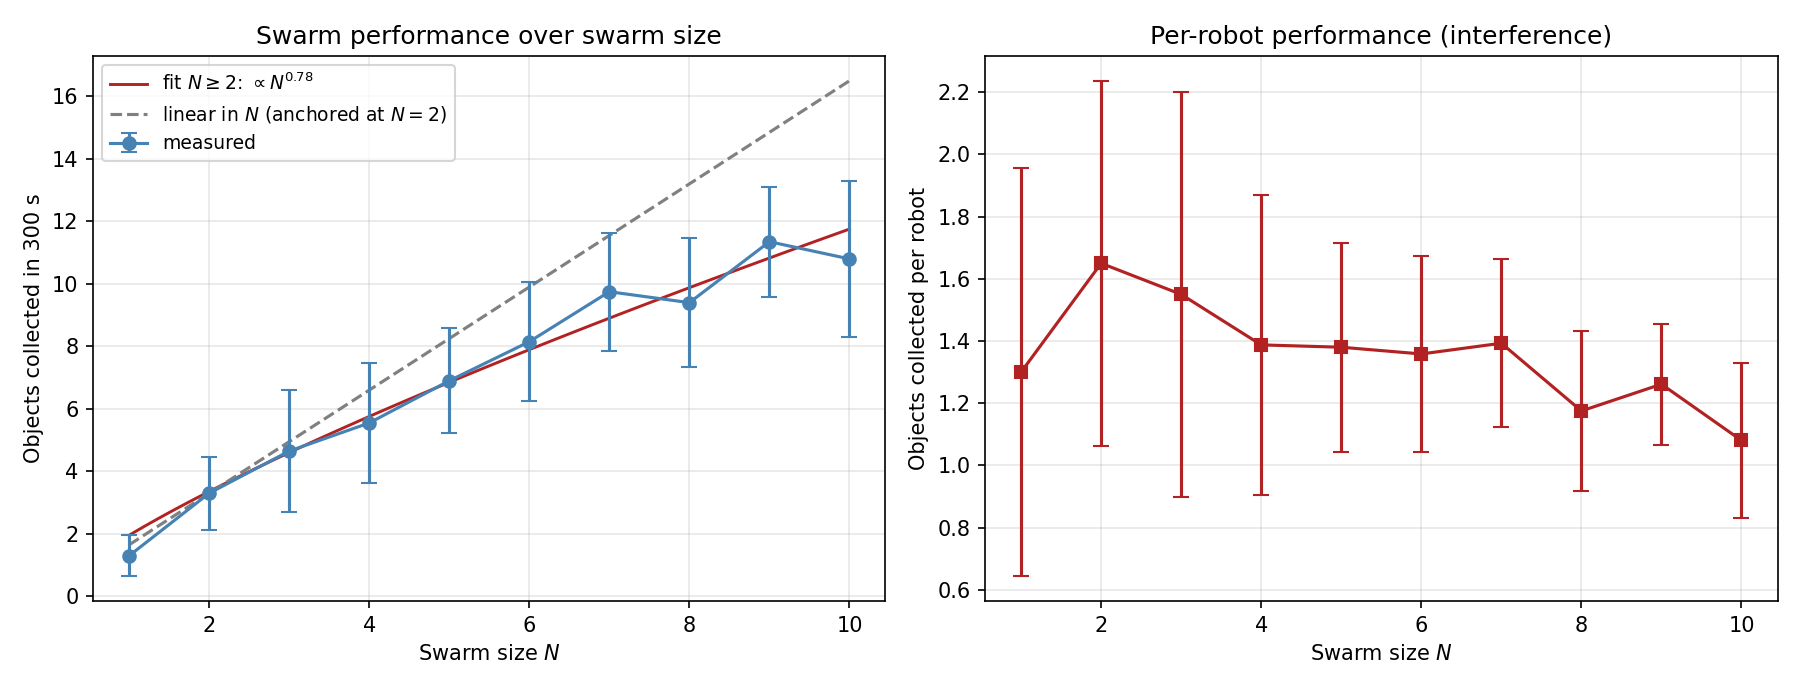
\includegraphics[width=\textwidth]{task_3/plots/task_3_performance.png}
    \caption{Left: swarm performance over swarm size, with a power-law fit over
             $N \ge 2$ and a linear reference anchored at $N = 2$.  Right:
             objects collected per robot.}
    \label{fig:task3-perf}
\end{figure}

\begin{figure}[h]
    \centering
    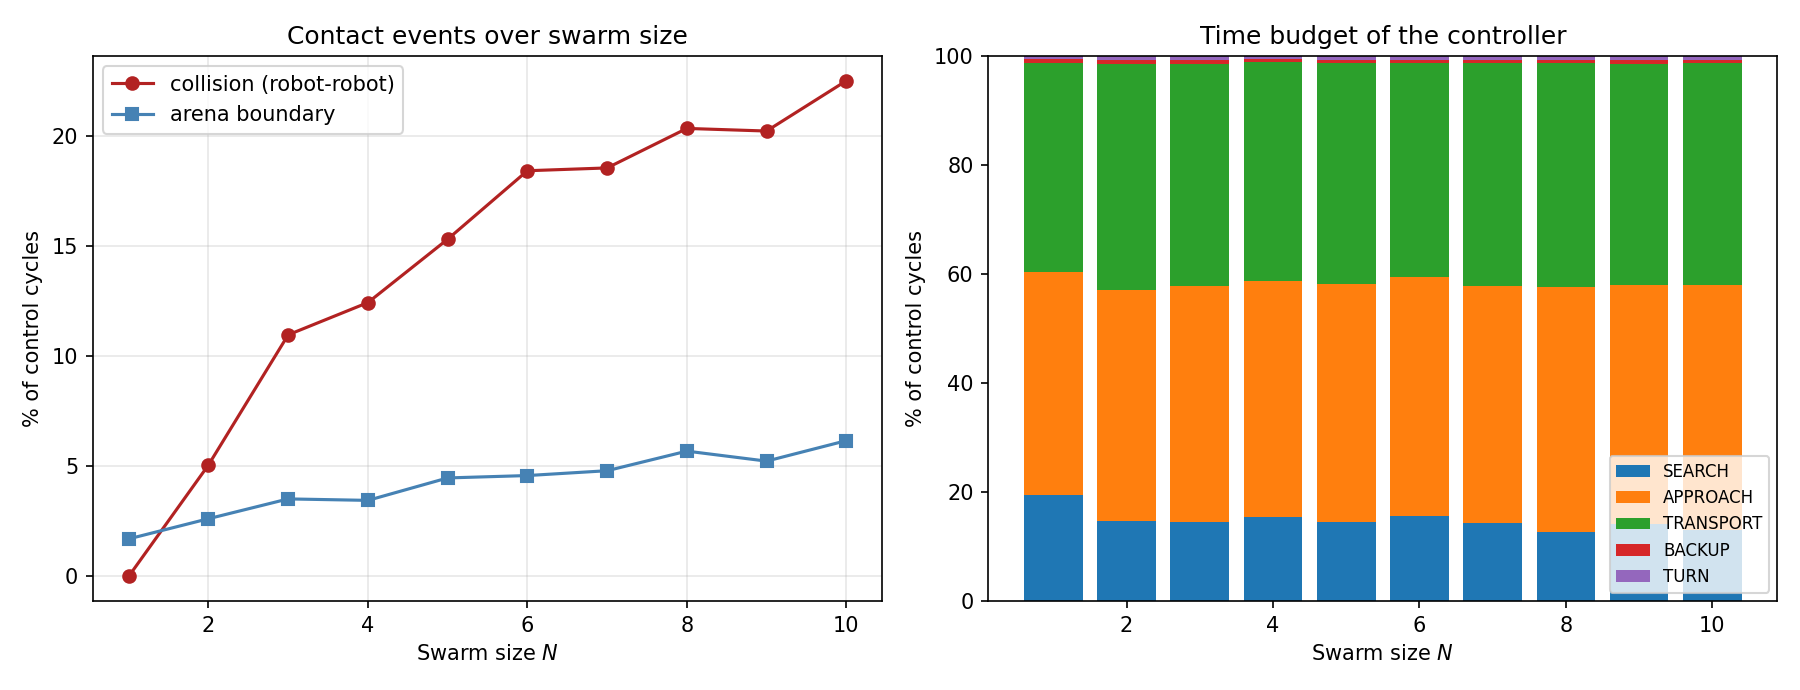
\includegraphics[width=\textwidth]{task_3/plots/task_3_behaviour.png}
    \caption{Left: fraction of control cycles reporting a robot--robot collision
             and an arena boundary.  Right: the controller's time budget.}
    \label{fig:task3-behav}
\end{figure}

\begin{figure}[h]
    \centering
    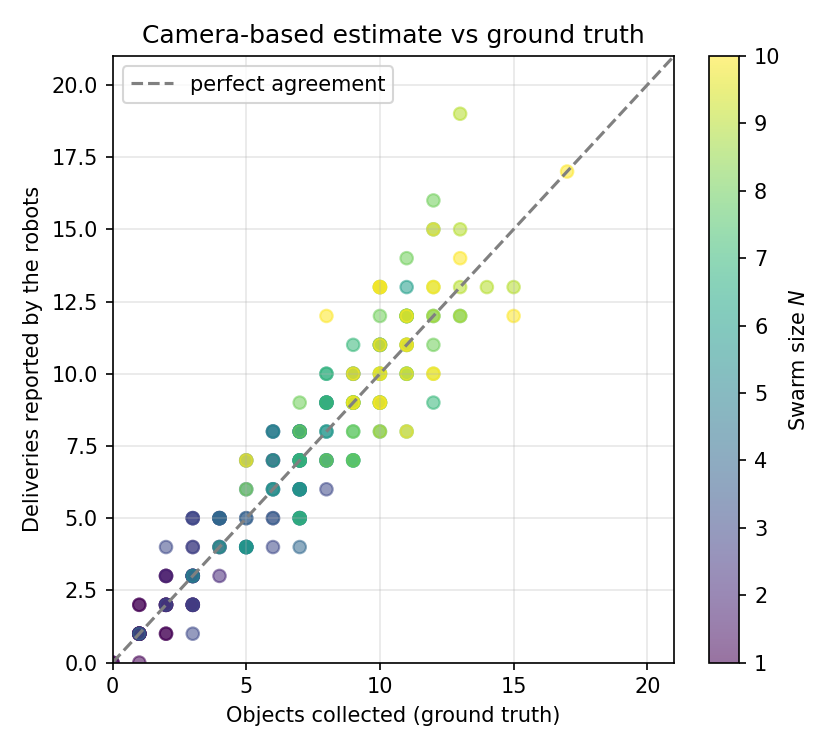
\includegraphics[width=0.6\textwidth]{task_3/plots/task_3_estimate_vs_truth.png}
    \caption{The robots' own camera-based delivery count against the ground
             truth measured by the loop functions, one point per run.}
    \label{fig:task3-truth}
\end{figure}

\paragraph{Performance is sublinear in the swarm size.}
The total number of collected objects grows from $1.3$ at $N = 1$ to $10.8$ at
$N = 10$, but not proportionally: a power-law fit over $N \ge 2$ gives
$\text{collected} \propto N^{0.78}$ (Figure~\ref{fig:task3-perf}, left).
Equivalently, per-robot performance falls from $1.65$ objects at $N = 2$ to
$1.08$ at $N = 10$, a loss of about a third.

\paragraph{The loss is interference.}
The fraction of control cycles in which a robot is in contact with another robot
rises almost linearly with the swarm size, from $0$ at $N = 1$ to $22.5\,\%$ at
$N = 10$ (Figure~\ref{fig:task3-behav}, left).  Encounters with the arena
boundary also rise, but far more slowly ($1.7\,\%$ to $6.2\,\%$), which is
expected: the arena does not change, only the number of robots in it does.
Meanwhile the controller's time budget is remarkably stable -- robots spend
${\approx}40\,\%$ of their cycles transporting at every swarm size
(Figure~\ref{fig:task3-behav}, right).  Robots in a larger swarm are therefore
not failing to find objects; they are spending their time pushing each other out
of the way while they do it.  This is the standard interference effect: the
arena is a shared, finite resource, and the cost of sharing it grows with the
number of robots.

\paragraph{A single robot is not a swarm of one.}
Per-robot performance \emph{rises} from $N = 1$ ($1.30$) to $N = 2$ ($1.65$)
before it begins to fall (Figure~\ref{fig:task3-perf}, right).  A lone robot has
no team-mate to happen upon an object it walked past, and when it gets stuck it
loses a large share of its $300$~s with nobody to compensate; the variance at
$N = 1$ is correspondingly the largest in the sweep.  For this reason we did not
draw the customary ``ideal linear'' reference through the single-robot rate,
which would place the measured curve \emph{above} the ideal and wrongly suggest
superlinear scaling.  We fit the exponent instead, and anchor the linear
reference at $N = 2$.

\paragraph{Self-reported performance is not trustworthy in general.}
After the fix described above, the robots' camera-based delivery count agrees
with the ground truth to within $2\,\%$ (Figure~\ref{fig:task3-truth}).  We
nevertheless score performance from the simulator, because that agreement is a
property of one carefully chosen light threshold and of the specific geometry of
this arena, not something a real swarm could rely on.  The general lesson is
that a swarm's own estimate of what it has achieved is a measurement like any
other, with its own bias, and it should be validated against ground truth before
it is used as a performance metric.

\subsection{Reproducing the Results}

\begin{lstlisting}[language=bash]
cd task_3
./run_docker.sh build         # build the ARGoS image (once)
./run_docker.sh loop          # compile the loop functions
./run_docker.sh gui           # watch one simulation
./run_docker.sh experiments   # the full sweep, ~3 min on 8 cores
./run_docker.sh plot          # write the figures
\end{lstlisting}

\newpage
% =============================================================================
\section{Completed Tasks}
% =============================================================================

\begin{center}
\begin{tabular}{lll}
\toprule
\textbf{Task} & \textbf{Description} & \textbf{Status} \\
\midrule
--- & Shared locust simulation, parameterised and vectorised    & \checkmark \\
--- & Verification against the tutorial-4 implementation        & \checkmark \\
\midrule
1 & Measurement of $\Delta L(L)$ over ${\approx}5000$ runs      & \\
1 & Plot of $\Delta L(L)$; meaning of the zeros $L^*$           & \\
1 & Fit of the swarm urn model ($c$ and $\varphi$)              & \\
1 & Plot of data, fit and $P_{FB}$                              & \\
\midrule
2 & Zone A/B/C bookkeeping, tested against known sequences      & \checkmark \\
2 & Sweep over swarm size ($10$ sizes, $2 \times 10^6$ steps each) & \checkmark \\
2 & Crossing time, waiting time and switch count over $N$       & \checkmark \\
2 & Reproduction of the density-dependent switching effect      & \checkmark \\
\midrule
3 & Foraging controller with the six required outputs           & \checkmark \\
3 & Bumper and pushing force emulated from proximity and camera & \checkmark \\
3 & Ground-truth scoring and object respawn (loop functions)    & \checkmark \\
3 & Sweep over swarm size $N = 1 \dots 10$ ($200$ runs)         & \checkmark \\
3 & Swarm performance over swarm size; interference analysis    & \checkmark \\
\bottomrule
\end{tabular}
\end{center}

\end{document}
